\documentclass[11pt]{article}
\usepackage[margin=1in]{geometry}
\usepackage[T1]{fontenc}
\usepackage{lmodern,microtype}
\usepackage{amsmath,amssymb,amsthm,mathtools,graphicx,booktabs}
\usepackage[dvipsnames]{xcolor}
\usepackage{hyperref}
\hypersetup{colorlinks=true,linkcolor=MidnightBlue,citecolor=MidnightBlue,urlcolor=MidnightBlue,
 pdftitle={Parity profiles for sampling without replacement}}
\setlength{\emergencystretch}{3em}
\newtheorem{theorem}{Theorem}
\newtheorem{lemma}[theorem]{Lemma}
\newtheorem{corollary}[theorem]{Corollary}
\newtheorem{remark}[theorem]{Remark}
\newcommand{\TV}{d_{\mathrm{TV}}}
\newcommand{\E}{\mathbb E}
\newcommand{\Pp}{\mathbb P}
\newcommand{\Var}{\operatorname{Var}}
\newcommand{\Law}{\mathcal L}
\newcommand{\PhiN}{\Phi}
\title{Parity profiles for sampling without replacement}
\author{Research continuation for Vladimir Reshetnikov's ProveIt project}
\date{27 November 2026}
\begin{document}
\maketitle

\begin{abstract}
Choose a fixed-size subset of $rn$ positions arranged in $r$ equal blocks,
and record only whether the occupancy of each block is odd or even.
For every sequence of capacities $n\ge2$, we prove that the joint parity
law is asymptotically equivalent in total variation to independent
biased signs conditioned on their product, whenever the single-block
binomial parity bias tends to zero. The exact parameter
$\sqrt r(1-2s/(rn))^n$ gives a Gaussian distance profile, including fixed
capacities and a finite-capacity correction to the classical hypercube
window. A self-contained local limit proof uses the negative real roots
of the even and odd sections of a binomial polynomial. The result
extends the finite-allocation analysis in ProveIt's GRH article;
an explicitly source-dependent corollary describes the transition for
many simultaneous prime products with a quadratic-character bias.
\end{abstract}

\section{Statement and scope}

The inspected source is ProveIt commit
\texttt{3413bfb1edb3636437f9cec7e5dd975869f7d120} \cite{ProveIt}.
All finite-population theorems in this paper are unconditional and are
proved below. The prime-factorization corollary separately identifies
its arithmetic input. These are ordinary mathematical proofs, not Lean
formalizations; their novelty relative to the source is distinguished
from the established Gaussian hypercube profile in the final section.

Partition $m=rn$ distinguishable slots into $r$ labelled blocks of equal size $n$.
Choose an $s$-element subset of the slots uniformly, let $H_i$ be its occupancy in
block $i$, and observe only $Y_i=(-1)^{H_i}$. Denote the law of
$Y=(Y_1,\ldots,Y_r)$ by $P_{r,n,s}$. Necessarily $\prod_iY_i=(-1)^s$.
For $\eta\in\{-1,1\}$ let $U_{r,\eta}$ be the uniform law on
$\{y\in\{-1,1\}^r:\prod_i y_i=\eta\}$.
For $0\le a<1$, let $Q_{r,a}$ have independent coordinates with
$Q(Y_i=1)=(1+a)/2$, and let $Q_{r,a}^{\eta}$ be this law conditioned on
$\prod_iY_i=\eta$.

\begin{theorem}[Equivalence after observing parities]\label{thm:equivalence}
Let $r\to\infty$, let $n=n_r\ge2$ be arbitrary integers, and let
$0\le s=s_r\le rn/2$ be integers. Put
\[
 p=\frac{s}{rn},\qquad t=1-2p,\qquad a=t^n,\qquad\eta=(-1)^s.
\]
If $a\to0$, then
\[
 \TV(P_{r,n,s},Q_{r,a}^{\eta})\longrightarrow0.
\]
There is no assumption that $n\to\infty$, nor that $s=o(rn)$.
\end{theorem}

\begin{theorem}[Complete critical profile]\label{thm:profile}
Under the hypotheses of Theorem~\ref{thm:equivalence}, if
$\sqrt r\,a\to\lambda\in[0,\infty]$, then
\[
 \TV(P_{r,n,s},U_{r,\eta})\longrightarrow
 F(\lambda):=2\PhiN(\lambda/2)-1,
\]
where $F(\infty)=1$ and $\PhiN$ is the standard normal distribution function.
For finite $\lambda$ the hypothesis $a\to0$ is automatic.
\end{theorem}

The restriction $n\ge2$ is essential. When $n=1$, the observed parity vector
determines the complete selected subset. At $s\sim r/2$ its support is one
Hamming layer, whose $U_{r,\eta}$-mass tends to zero, so the total variation
distance tends to one even when $\sqrt r\,a\to0$.

\section{An elementary local limit lemma}

\begin{lemma}[Local limit for arbitrary Bernoulli sums]\label{lem:llt}
Let $Z=\sum_{j=1}^N B_j$ be a sum of independent Bernoulli random variables,
whose probabilities may be unequal and may depend on the member of a sequence.
Write $\mu=\E Z$ and $v=\Var Z$. If $v\to\infty$, then
\[
 \sup_{k\in\mathbb Z}\left|\sqrt v\,\Pp(Z=k)
 -\frac1{\sqrt{2\pi}}\exp\left(-\frac{(k-\mu)^2}{2v}\right)\right|\to0.
\]
The convergence is uniform over all finite Bernoulli arrays with $v\to\infty$.
\end{lemma}

\begin{proof}
The modulus of the characteristic function satisfies
\[
 |\E e^{i\theta(Z-\mu)}|
 \le\exp\{-2v\sin^2(\theta/2)\},\qquad |\theta|\le\pi.
\]
Indeed, the squared modulus of one Bernoulli factor is
$1-4u(1-u)\sin^2(\theta/2)$, and $1-x\le e^{-x}$.
For fixed $w$, the centered characteristic function at $\theta=w/\sqrt v$
converges to $e^{-w^2/2}$ uniformly in the arrays: the sum of the centered
third absolute moments is at most $v$, and the Taylor remainder is
$O(|w|^3/\sqrt v)$, with the logarithmic correction controlled in the same way.
After rescaling the inversion integral by $w=\sqrt v\,\theta$, the preceding
modulus bound is at most $e^{-2w^2/\pi^2}$ on $|w|\le\pi\sqrt v$, since
$\sin(|\theta|/2)\ge|\theta|/\pi$. Extend the integrand by zero outside that
interval. Dominated convergence makes its $L^1$-difference from
$e^{-w^2/2}$ tend to zero. Fourier inversion and the normal inversion formula
then give the displayed bound, uniformly in the phase
$e^{-iw(k-\mu)/\sqrt v}$ and hence uniformly in $k$.
\end{proof}

\begin{lemma}[A binomial conditioned on its parity]\label{lem:roots}
If $W\sim\operatorname{Bin}(n,p)$ with $n\ge1$ and $0<p<1$, then, conditional on either
parity $e\in\{0,1\}$, $W$ has the law
\[
 e+2\sum_j B_j
\]
for some independent Bernoulli variables. Empty sums are permitted.
\end{lemma}

\begin{proof}
Put $q=1-p$ and consider
\[
 E_n(z)=\sum_k\binom n{2k}q^{n-2k}p^{2k}z^k,
 \quad
 O_n(z)=\sum_k\binom n{2k+1}q^{n-2k-1}p^{2k+1}z^k.
\]
These are the unnormalized probability generating polynomials for $W/2$
given $W$ even and $(W-1)/2$ given $W$ odd. All their zeros are real and
strictly negative. To see this directly, put $z=w^2$ and use
\[
 2E_n(w^2)=(q+pw)^n+(q-pw)^n,
 \qquad
 2wO_n(w^2)=(q+pw)^n-(q-pw)^n.
\]
At a nonzero root the ratio $(q+pw)/(q-pw)$ is an $n$th root of $-1$ or
$1$, respectively. Solving for $w$ gives a purely imaginary number, since
$(\zeta-1)/(\zeta+1)$ is purely imaginary for $|\zeta|=1$, $\zeta\ne-1$.
The excluded value $\zeta=-1$ corresponds to the missing highest-degree
term rather than a finite root; the root $w=0$ in the odd numerator is
removed by division by $w$. Explicitly the roots are
\[
 -\left(\frac qp\right)^2\tan^2\frac{(2j-1)\pi}{2n},
 \quad 1\le j\le\lfloor n/2\rfloor,
\]
for $E_n$, and
\[
 -\left(\frac qp\right)^2\tan^2\frac{j\pi}{n},
 \quad 1\le j\le\lfloor(n-1)/2\rfloor,
\]
for $O_n$. These lists contain all roots. Positive coefficients and nonzero constants exclude
zero and positive roots. A polynomial with positive constant term and
negative real roots, normalized to have value one at $z=1$, factors as
$\prod_j(1-\beta_j+\beta_j z)$ with $0<\beta_j<1$.
\end{proof}

\section{Proof of equivalence of the parity laws}

Let $W_1,\ldots,W_r$ be independent $\operatorname{Bin}(n,p)$ variables,
$T=\sum_iW_i$, and $Y_i=(-1)^{W_i}$. Conditional on $T=s$, the underlying
$rn$ Bernoulli choices form a uniform $s$-subset; therefore the law of
$Y\mid T=s$ is exactly $P_{r,n,s}$. Before conditioning, $Y$ has law
$Q_{r,a}$.

Set $b=np(1-p)$, and define
\[
 u=-2b t^{n-1},\qquad
 v=-2ba+4b^2(1-1/n)t^{n-2}.
\]
The expressions at $t=0$ have their usual polynomial meanings; in
particular $t^0=1$. The moment generating function of one binomial
conditioned on $Y_i=y_i$ is
\[
 (1-p+pe^z)^n\,
 \frac{1+y_i\left(\dfrac{1-p-pe^z}{1-p+pe^z}\right)^n}{1+y_i a}.
\]
Differentiating its logarithm twice at zero gives
\[
 \E(W_i\mid Y_i=y_i)=np+\frac{y_i u}{1+y_i a},\qquad
 \Var(W_i\mid Y_i=y_i)=b+\frac{y_i v}{1+y_i a}
 -\frac{u^2}{(1+y_i a)^2}.
\]
Consequently, writing $J=\sum_i y_i$, the conditional mean $\mu_y$ and
variance $V_y$ of $T$ satisfy the exact formulas
\begin{align}
 \mu_y-s&=u\frac{J-ra}{1-a^2},\label{eq:mean}\\
 V_y&=rb+v\frac{J-ra}{1-a^2}
 -u^2\frac{r(1+a^2)-2aJ}{(1-a^2)^2}.\label{eq:var}
\end{align}

The following three elementary bounds are uniform for every $n\ge2$ and
$0\le t<1$:
\begin{align}
 b&\ge\frac{1-a}{4},\label{eq:b-lower}\\
 b t^{n-2}&\le\frac12,\label{eq:b-root}\\
 b t^{2n-2}&\le-\frac12a\log a,\label{eq:b-small}
\end{align}
where the right side in the last display is zero at $a=0$. For
\eqref{eq:b-lower}, use $1-t^n\le n(1-t)=2np$ and $1-p\ge1/2$.
For \eqref{eq:b-root}, put $z=t^2$ and $h=n/2\ge1$; then
$bt^{n-2}=\tfrac12h(1-z)z^{h-1}\le1/2$ by maximizing the displayed
elementary function (the case $h=1$ is immediate). For
\eqref{eq:b-small}, $n(1-z)\le-n\log z=-2\log a$, while
$z^{n-1}=a^{2-2/n}\le a$ because $n\ge2$.
In particular $|v|\le4b$ and $bt^{2n-2}\to0$ whenever $a\to0$.

Fix $M>0$ and restrict to
\[
 \mathcal T_M=\{y:|J-ra|\le M\sqrt r\}.
\]
Under $Q_{r,a}$, $J$ has variance $r(1-a^2)$, so Chebyshev gives
$Q_{r,a}(\mathcal T_M^c)\le M^{-2}$. Since
\[
 Q_{r,a}(\textstyle\prod_iY_i=\eta)=\frac{1+\eta a^r}{2}\to\frac12,
\]
the conditioned probability of this complement is at most
$(2+o(1))M^{-2}$.
Uniformly on $\mathcal T_M$, equations \eqref{eq:mean}--\eqref{eq:var}
and the elementary bounds imply
\[
 \frac{|\mu_y-s|}{\sqrt{rb}}
 \le\frac{2M\sqrt b\,t^{n-1}}{1-a^2}=o(1),
 \qquad
 \frac{V_y}{rb}=1+o(1).
\]
For the variance, the linear term contributes at most
$4M/((1-a^2)\sqrt r)$ relatively, and the final term at most
$4bt^{2n-2}/(1-a)^2=o(1)$. Also $rb\to\infty$ by
\eqref{eq:b-lower}.

Given $Y=y$, the $W_i$ remain independent. By Lemma~\ref{lem:roots},
$T\mid Y=y$ is an integer offset plus twice a sum of independent Bernoulli
variables, whose variance is $V_y/4$. Its offset has the same parity as
$s$ whenever $\prod_i y_i=\eta$. Lemma~\ref{lem:llt} therefore gives,
uniformly over such $y\in\mathcal T_M$,
\[
 \Pp(T=s\mid Y=y)=\frac{2+o(1)}{\sqrt{2\pi rb}}.
\]
The unconditioned $T$ is $\operatorname{Bin}(rn,p)$ with mean exactly $s$
and variance $rb$, so the same local limit lemma gives
\[
 \Pp(T=s)=\frac{1+o(1)}{\sqrt{2\pi rb}}.
\]
The likelihood ratio on the parity fibre is thus
\[
 \frac{P_{r,n,s}(y)}{Q_{r,a}^{\eta}(y)}
 =\frac{1+\eta a^r}{2}
 \frac{\Pp(T=s\mid Y=y)}{\Pp(T=s)}=1+o(1)
\]
uniformly on every fixed typical set $\mathcal T_M$. Letting $M\to\infty$
shows that this likelihood ratio tends to one in
$Q_{r,a}^{\eta}$-probability. Since its expectation is one,
\[
 \TV(P,Q)=1-\E_Q\min\{dP/dQ,1\}\longrightarrow0.
\]
This proves Theorem~\ref{thm:equivalence} without any full-occupancy
independent-placement approximation.

\section{Proof of the Gaussian profile}

The likelihood ratio of $Q_{r,a}^{\eta}$ with respect to $U_{r,\eta}$ is
\[
 L(y)=\frac{\prod_{i=1}^r(1+a y_i)}{1+\eta a^r}.
\]
Under $U_{r,\eta}$, the normalized sum $J/\sqrt r$ tends to $N(0,1)$.
One elementary proof is to take $r-1$ independent fair signs and make the
last sign their product times $\eta$; the last sign changes the normalized
sum by at most $1/\sqrt r$.
If $\sqrt r\,a\to\lambda<\infty$, then uniformly in $y$
\[
 \log L(y)=aJ-\frac{ra^2}{2}+O(ra^3)-\log(1+\eta a^r)
 \ \Longrightarrow\ \lambda Z-\lambda^2/2,
 \quad Z\sim N(0,1).
\]
The bounded continuous function $x\mapsto(1-e^x)_+$ yields
\[
 \TV(Q_{r,a}^{\eta},U_{r,\eta})
 =\E_{U_{r,\eta}}(1-L)_+
 \longrightarrow \E(1-e^{\lambda Z-\lambda^2/2})_+
 =2\PhiN(\lambda/2)-1.
\]
The last integral follows by splitting at $Z=\lambda/2$ and completing
the square in the tilted normal density.

If $a\to0$ but $\sqrt r\,a\to\infty$, the event $J>ra/2$ has
$Q_{r,a}^{\eta}$-probability tending to one and $U_{r,\eta}$-probability
tending to zero, by Chebyshev and the conditioning probability tending to
$1/2$. Hence the distance tends to one. The triangle inequality with
Theorem~\ref{thm:equivalence} proves Theorem~\ref{thm:profile}.

\section{Capacity effects and correct windows}

The level $\lambda=1$ is located at
\[
 s_*(r,n)=\frac{rn}{2}\left(1-r^{-1/(2n)}\right).
\]
The nonlinear clock
\[
 s(c)=\frac{rn}{2}\left(1-e^{-2c/n}r^{-1/(2n)}\right)
\]
has $\sqrt r\,a=e^{-2c}$ exactly before integer rounding. Rounding changes
the logarithm of $\sqrt r\,a$ by $o(1)$ for all $n\ge2$, because
$r r^{-1/(2n)}\ge r^{3/4}\to\infty$. Thus its limiting profile is
$2\PhiN(e^{-2c}/2)-1$ for every fixed real $c$.

If $n\to\infty$, the linear scale
$s=s_*(r,n)+c r\delta$, $\delta=r^{-1/(2n)}$, has the same limiting
$\lambda=e^{-2c}$. If in addition $n\gg(\log r)^2$, then
\[
 s_* = \frac r4\log r-\frac{r(\log r)^2}{16n}
 +O\left(\frac{r(\log r)^3}{n^2}\right),\qquad\delta\to1,
\]
and the classical hypercube centre $r\log r/4$ and window $r$ apply.
If $n/(\log r)^2\to\kappa\in(0,\infty)$, then at
$s=r\log r/4+cr$ the parameter instead converges to
$\lambda=e^{-2c-1/(8\kappa)}$. The finite capacity therefore shifts the
profile by a nonvanishing amount on the classical window.

For fixed $n\ge2$, the proper description is a central mixing valley:
at $s=rn/2-u r^{1-1/(2n)}+O(1)$ with fixed $u\ge0$,
\[
 \TV(P_{r,n,s},U_{r,(-1)^s})\longrightarrow
 2\PhiN\left(\frac12(2u/n)^n\right)-1.
\]
For sample sizes above $rn/2$, complementing the selected subset changes
every sign by $(-1)^n$ and gives the identical distance with $s$ replaced
by $rn-s$. Thus one must not claim ordinary monotone Markov-chain mixing
for this finite sampling process: after the central region the distance
increases again, ending at a point mass when all slots are selected.

\section{General entropy improvement}

For $B$ nonempty boxes of arbitrary capacities $n_i$, $m=\sum_i n_i\ge2$,
consider the box labels of $s$ distinct uniform slots. Let $P$ be their
joint ordered law and let $Q$ have independent box labels with
probabilities $\alpha_i=n_i/m$. Then
\[
 D(P\Vert Q)\le(B-1)\sum_{\ell=0}^{s-1}
 \frac{\ell}{(m-1)(m-\ell)},\qquad
 \TV(P,Q)\le\sqrt{\frac{B-1}{2}
 \sum_{\ell=0}^{s-1}\frac{\ell}{(m-1)(m-\ell)}}.
\]
Indeed, after $\ell$ draws with occupancies $H_i$, the conditional next
probabilities are $(n_i-H_i)/(m-\ell)$. The relative entropy is at most
the chi-square divergence against $\alpha$; the expected divergence is
\[
 \sum_i\frac{\Var(H_i)}{\alpha_i(m-\ell)^2}
 =\frac{\ell}{(m-1)(m-\ell)}\sum_i(1-\alpha_i)
 =\frac{(B-1)\ell}{(m-1)(m-\ell)}.
\]
Use the hypergeometric variance, the entropy chain rule, and Pinsker's
inequality. Any deterministic function of the labels, including arbitrary
finite-group colour sums, obeys the same total variation bound.
In particular, for $s\le m$,
\[
 \TV(P,Q)\le\frac{\sqrt{(B-1)s(s-1)}}
 {2\sqrt{(m-1)(m-s+1)}}.
\]
This improves the collision coupling $s(s-1)/(2m)$ in many growing-box
regimes, but the parity theorem above remains valid far beyond either
full-label approximation regime.
If $m=1$, the two label laws coincide and their distance is zero.

\section{A source-dependent prime-factorization consequence}

The following consequence uses, in addition to Dirichlet GRH, the
uniform-lifting theorem \path{dir:thm:disjoint-growing} in the repository
article. That arithmetic theorem is an input here, not independently
reproved by this note. The preceding finite-population results are
unconditional and independent of that input.

Fix a retained-density constant $\alpha\in(1/3,1/2)$ and use the constants
$B,C$ supplied by the source theorem (with any fixed power-saving exponent
$A>0$). Let $q\to\infty$, $L=\log q$, $G=(\mathbb Z/q\mathbb Z)^\times$,
and let $\mathcal P_q$ be the primes at most $CL^2$ not dividing $q$.
Let $S\subseteq\mathcal P_q$ have $m=rn\ge\alpha|\mathcal P_q|$, with
$r\to\infty$ and $n\ge BL$. Partition $S$ uniformly into $r$ labelled
blocks of $n$ primes. Write $X_i$ for their products modulo $q$ and
$P_S=\prod_{p\in S}p\pmod q$.
Let $\chi$ be a nonprincipal quadratic character, let $\sigma\in\{-1,1\}$,
and suppose exactly $s$ members of $S$ have $\chi(p)=-\sigma$.

\begin{corollary}[Growing quadratic factorization profile]\label{cor:arithmetic}
In this setting, for fixed $c\in\mathbb R$, suppose
\[
 s=\frac r4\log r+cr+o(r).
\]
If $\mathcal U_q$ is uniform on the compatibility set
\[
 \{(g_1,\ldots,g_r)\in G^r:\textstyle\prod_i g_i=P_S\},
\]
then
\[
 \TV(\Law(X_1,\ldots,X_r),\mathcal U_q)
 \longrightarrow 2\PhiN(e^{-2c}/2)-1.
\]
This holds throughout the growing range allowed by the source theorem,
including $r$ of order $L/\log L$ whenever the displayed hypotheses hold.
\end{corollary}

\begin{proof}
The source uses a reserve block and $r-1$ recorded blocks; take one of the
$r$ equal blocks as reserve. The recorded residue tuple determines the
reserve residue through $P_S$, so this change of presentation is a
bijection of the compatibility set. Since $|\mathcal P_q|=O(L^2/\log L)$
and $n\ge BL$, one has $r=O(L/\log L)$ and $n\gg(\log r)^2$.
Thus $s/m=O(\log r/n)\to0$. The character $\chi$ has retained-set bias
$1-2s/m\to1$, so it belongs to the source's high-bias subgroup $H_\tau$
for all sufficiently large $q$. That subgroup has order at most
$\lfloor1/\alpha\rfloor=2$; hence $H_\tau=\langle\chi\rangle$.

The corrected signs $Y_i=\sigma^n\chi(X_i)$ have exactly the finite-slot
parity law $P_{r,n,s}$. Source uniform lifting makes the residue law
differ in total variation by at most $q^{-A}/2$ from the uniform lift of
this parity law. Uniform lifting over equal-sized fibres preserves total
variation, and the uniform compatibility law lifts $U_{r,(-1)^s}$.
Finally, writing $t=1-2s/(rn)$,
\[
 \log(\sqrt r\,t^n)
 =\frac12\log r-\frac{2s}{r}
 +O\left(\frac{s^2}{r^2n}\right)\longrightarrow-2c.
\]
Apply Theorem~\ref{thm:profile} and the triangle inequality.
\end{proof}

At $r\asymp L/\log L$, this transition uses $s\asymp L$ exceptions
while $m\asymp L^2/\log L$. Thus $s^2/m\asymp\log L$, and the source's
collision-coupling error does not tend to zero. The entropy improvement
already suffices in this arithmetic range; the stronger finite-population
parity theorem also covers fixed block capacities that cannot occur
under these arithmetic quota requirements. This corollary treats the
rank-one quadratic quotient, not all cyclic-four or Klein-four quotient
laws at retained density one quarter.

\section{Exact finite verification}

The included \texttt{checks/verify\_parity.py} computes the full law of
the number of odd blocks by integer coefficient extraction. For a fixed
set of $k$ odd blocks its count is the coefficient of $z^s$ in
\[
 \left(\sum_{j\ \mathrm{odd}}\binom njz^j\right)^k
 \left(\sum_{j\ \mathrm{even}}\binom njz^j\right)^{r-k}.
\]
Multiplication by $\binom rk$ and division by $\binom{rn}s$ gives the
probability of exactly $k$ odd blocks. Both this law and the comparison
laws are exchangeable, so total variation of the entire vector equals
total variation of these one-dimensional counts. The program verifies
56 small parameter cases against full subset enumeration and computes
95 larger profile cases. Counts and the distance from the uniform
parity fibre are exact; comparisons to the Gaussian and conditioned-iid
laws use floating-point evaluation and are illustrations, not proof.

\begin{figure}[htbp]
 \centering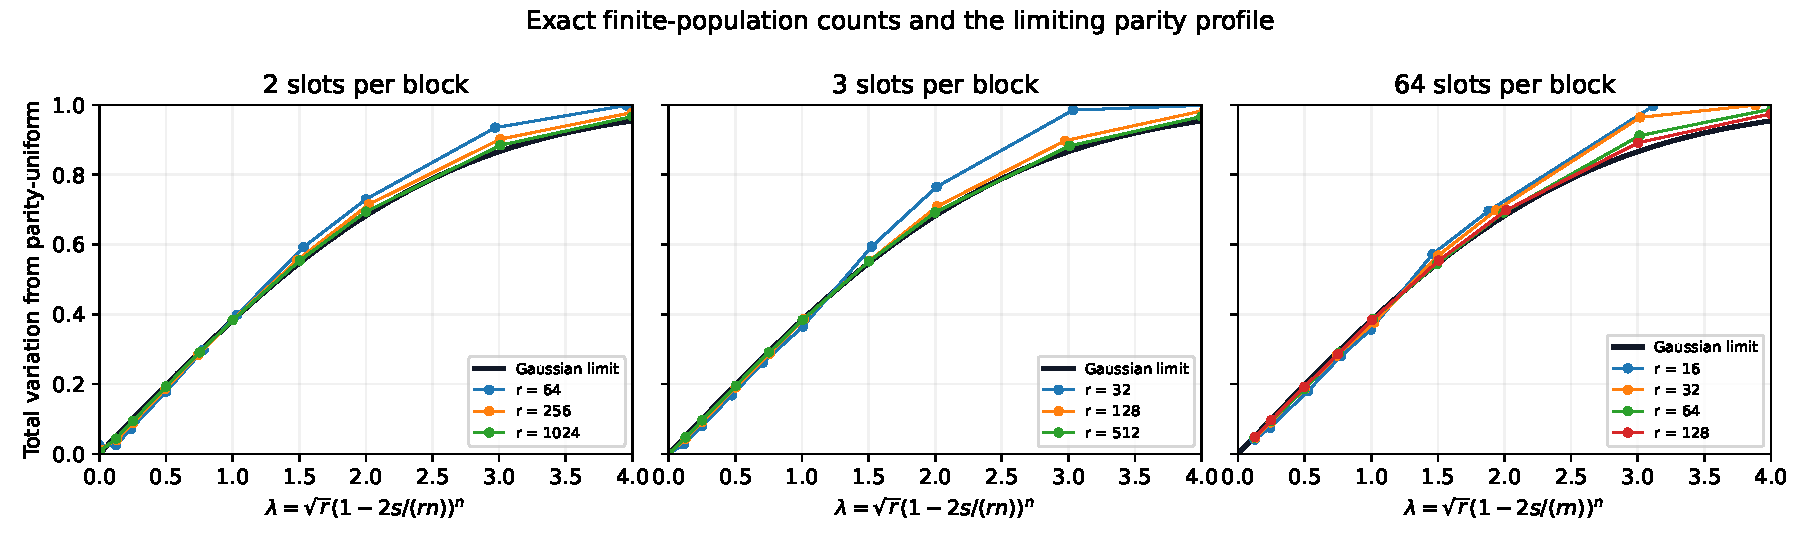
\includegraphics[width=\textwidth]{figures/parity_profile.pdf}
 \caption{Exact finite-population parity counts approach the common profile
 $2\Phi(\lambda/2)-1$. The three panels cover fixed capacities two and
 three and a larger capacity.}
\end{figure}

\section{Prior-work positioning}

The Gaussian cutoff shape for ordinary hypercube random walks is
classical and is not claimed as new. A primary reference is
P. Diaconis, R. L. Graham and J. A. Morrison,
\emph{Asymptotic analysis of a random walk on a hypercube with many
dimensions}, Random Structures and Algorithms 1 (1990), 51--72,
\href{https://doi.org/10.1002/rsa.3240010105}{doi:10.1002/rsa.3240010105}.
An author-hosted copy is at
\url{https://fanchung.ucsd.edu/ron/papers/90_02_hypercube_random_walk.pdf}.
The candidate new contribution here is the capacity-uniform finite-slice
parity equivalence for every $n_r\ge2$, its exact finite-population
parameter, and the resulting fixed-capacity and intermediate-capacity
profiles. Targeted searches did not locate this exact theorem; that is
not proof of bibliographic novelty. Alves et al.\ \cite{Alves} study a
related sampling-without-replacement comparison for a fixed number of
suits, retaining the full label sequence. Our theorem observes only
parities, lets the number of blocks grow, and allows every sequence of
block capacities at least two; it is a different comparison.

The ProveIt source connection is
\texttt{Article/sections/dir.tex}, labels
\texttt{dir:lem:disjoint-iid}, \texttt{dir:prop:sparseexc}, and
\texttt{dir:thm:disjoint-growing}. The first already contains the
fixed-block entropy calculation; retaining its dependence on the number
of boxes gives the general bound above. The finite-slice parity theorem
does not follow from the existing collision bound and uses no GRH.
The arithmetic corollary above composes it with the source's uniform
lifting theorem, retaining its hypotheses and using $r$ for the total
number of equal blocks, including the reserve.

The same pinned repository contains the incoming report \emph{Every sparse
prime-product transition is compound Poisson} \cite{IncomingCP}. It classifies
one sparse sampled product in a bounded quotient and develops a signed-measure
finite-population correction in a bounded expected-defect window. Its quotient
order stays bounded at fixed retained density; here the compatible parity
space has size $2^{r-1}$ and $r\to\infty$. Our theorem also permits fixed block
capacities and sampling fractions tending to one half, outside that report's
sparse-quota classification. Encoding the full parity vector in $C_2^r$ does
not put it within the stated defect expansion: all slots then carry a
nonidentity basis vector, and translating one colour to the identity still
leaves $rn-n>rn/2$ defects when $r>2$. The new theorem is the joint parity
equivalence under only $a\to0$, not the existing bounded-quotient reduction,
compound-Poisson mechanism, or the classical Gaussian profile.

\begin{thebibliography}{9}
\raggedright
\bibitem{ProveIt}
V. Reshetnikov, \emph{ProveIt: Analysis/GeneralizedRiemannHypothesis},
commit \texttt{3413bfb1edb3636437f9cec7e5dd975869f7d120},
inspected 27 November 2026.
\href{https://github.com/VladimirReshetnikov/ProveIt/blob/3413bfb1edb3636437f9cec7e5dd975869f7d120/Analysis/GeneralizedRiemannHypothesis/Article/sections/dir.tex}{Pinned arithmetic section},
particularly \texttt{dir:thm:disjoint-growing} and
\texttt{dir:prop:sparseexc}.
\bibitem{DGM}
P. Diaconis, R. L. Graham and J. A. Morrison,
Asymptotic analysis of a random walk on a hypercube with many dimensions,
\emph{Random Structures \& Algorithms} \textbf{1} (1990), 51--72.
\href{https://doi.org/10.1002/rsa.3240010105}{doi:10.1002/rsa.3240010105}.
\bibitem{Alves}
R. Alves, S. Est\'acio, S. Fr\'ometa, M. Jara, R. Marinho,
L. F. S. Marques and J. V. A. Pimenta,
\emph{Simulating simple random walks with a deck of cards},
arXiv:2410.00831v2 (2024). \url{https://arxiv.org/html/2410.00831v2}.
\bibitem{IncomingCP}
ProveIt research report, \emph{Every sparse prime-product transition is
compound Poisson: bounded quotients, a sharp mixing criterion, and a uniform
finite-population correction}, 27 November 2026. File
\texttt{grh\_extensions/prime\_product\_limits.tex} inside the incoming archive
\texttt{grh\_extensions\_2026-11-27(2).zip}, at the pinned revision above.
\href{https://github.com/VladimirReshetnikov/ProveIt/blob/3413bfb1edb3636437f9cec7e5dd975869f7d120/Analysis/GeneralizedRiemannHypothesis/docs/incoming/grh_extensions_2026-11-27(2).zip}{Pinned incoming report}.
\end{thebibliography}
\end{document}
